
\begin{frame}{软件设计目标}

我们希望开发一个简单易用且高效的软件平台环境, 集成重用已有研究成果, 提高项目组科研和教学效率。

软件适用对象:

\begin{itemize}
\tightlist
\item
  从事计算数学研究的科研工作者
\item
  计算数学专业的研究生
\end{itemize}
\end{frmae}

\begin{frame}{软件特色}

集成湘大已有的丰富研究成果:
\begin{itemize}
\tightlist
\item
  超收敛
\item
  快速算法
\item
  网格生成与优化
\item
  电磁场计算
\item
  高分子数值模拟
\end{itemize}
\end{frame}


\begin{frame}{架构设计}
\only<1>{
\begin{itemize}
\tightlist
\item
  以 Python 3 为主要开发语言, C++ 为辅助开发语言
\item
  面向数组和面向对象的编程模式
\item
  以成熟的 Python 科学计算与可视化模块为基础

  \begin{itemize}
  \tightlist
  \item
    numpy: https://www.numpy.org 多维数组及运算功能.
  \item
    scipy: https://www.scipy.org 稀疏矩阵及运算、
    最优化等科学计算等功能。
  \item
    matplotlib: http://matplotlib.org 画图功能
  \item
    mpi4py: https://mpi4py.scipy.org MPI for Python
  \item
    pycuda: NVDIA CUDA 并行计算 Python 接口
  \end{itemize}
\end{itemize}
}
\only<2>{
\begin{figure}[htbp]
\centering
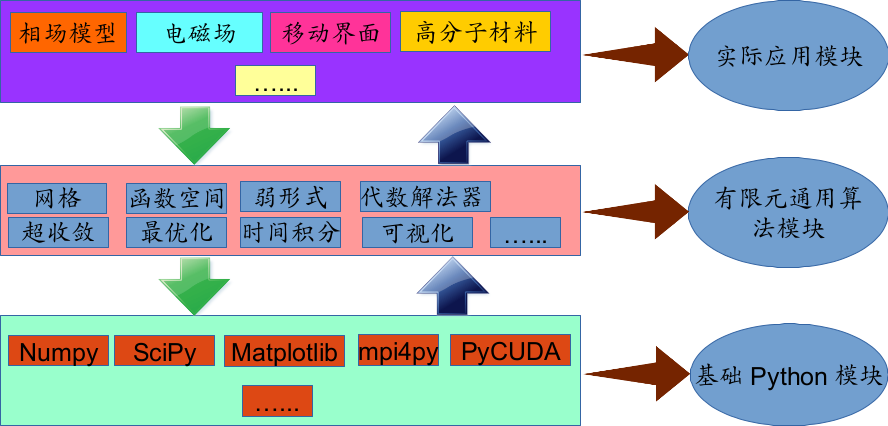
\includegraphics{./sa.png}
\caption{基于 Python 3 软件架构设计.}
\end{figure}
}
\end{frame}

\begin{frame}{已实现功能}
\begin{itemize}
\tightlist
\item
  简单区域上的结构网格生成与一致加密
\item
  隐函数表示区域上非结构网格生成和优化.
\item
  三角形网格上任意次 Lagrangian 有限元空间
\item
  Laplace 算子的和源项的弱形式
\item
  四阶问题的恢复型弱形式
\item
  Dirichlet 边界条件的处理
\item
  与代数多重网格解法器 pyamg 的接口
\end{itemize}
\end{frame}

\frame{frame}{下一步工作}

目前, 我们的软件包的设计和实现还很初步, 还有很多优化和改进的空间,
下一步我们会为增加更多的功能, 如:

\begin{itemize}
\tightlist
\item
  二分法自适应加密算法
\item
  支持更多的网格类型, 如四边形, 多边形, 四面体和多面体网格的网格类型
\item
  网格并行优化功能
\item
  实现更多的有限元空间, 如混合有限元空间, 虚单元法有限元空间等
\item
  \ldots{}\ldots{}
\end{itemize}
\end{frame}

